\subsection{Tiling}

\frame{
  \frametitle{Representing Collision Strings}

  \begin{itemize}
    \item Reflect squares about each side to create a tiling
    \item Solutions become lines in the plane
    \item Intersections become places where collisions occur
  \end{itemize}
}

\frame{
  \frametitle{Representing Collision Strings}

  \begin{example}
    Tiling of $\vec{x}_0 = (0, 0.5)$ and $\vec{v} = (0.25, 0.25)$.
  \end{example}

  \begin{columns}
    \begin{column}{0.45\textwidth}
      \begin{figure}
        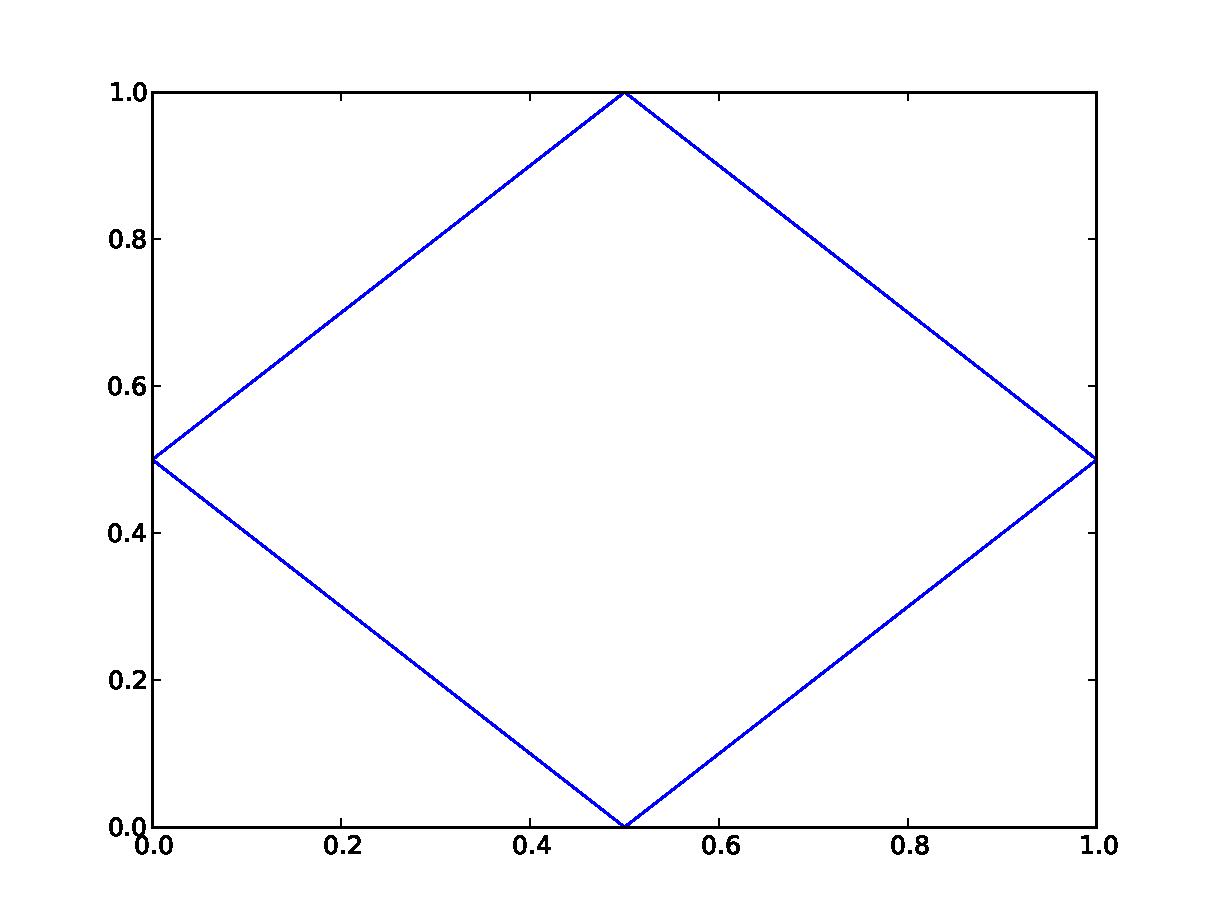
\includegraphics[width=2.1in]{abab.pdf}
      \end{figure}
    \end{column}
    \begin{column}{0.45\textwidth}
      \begin{figure}
        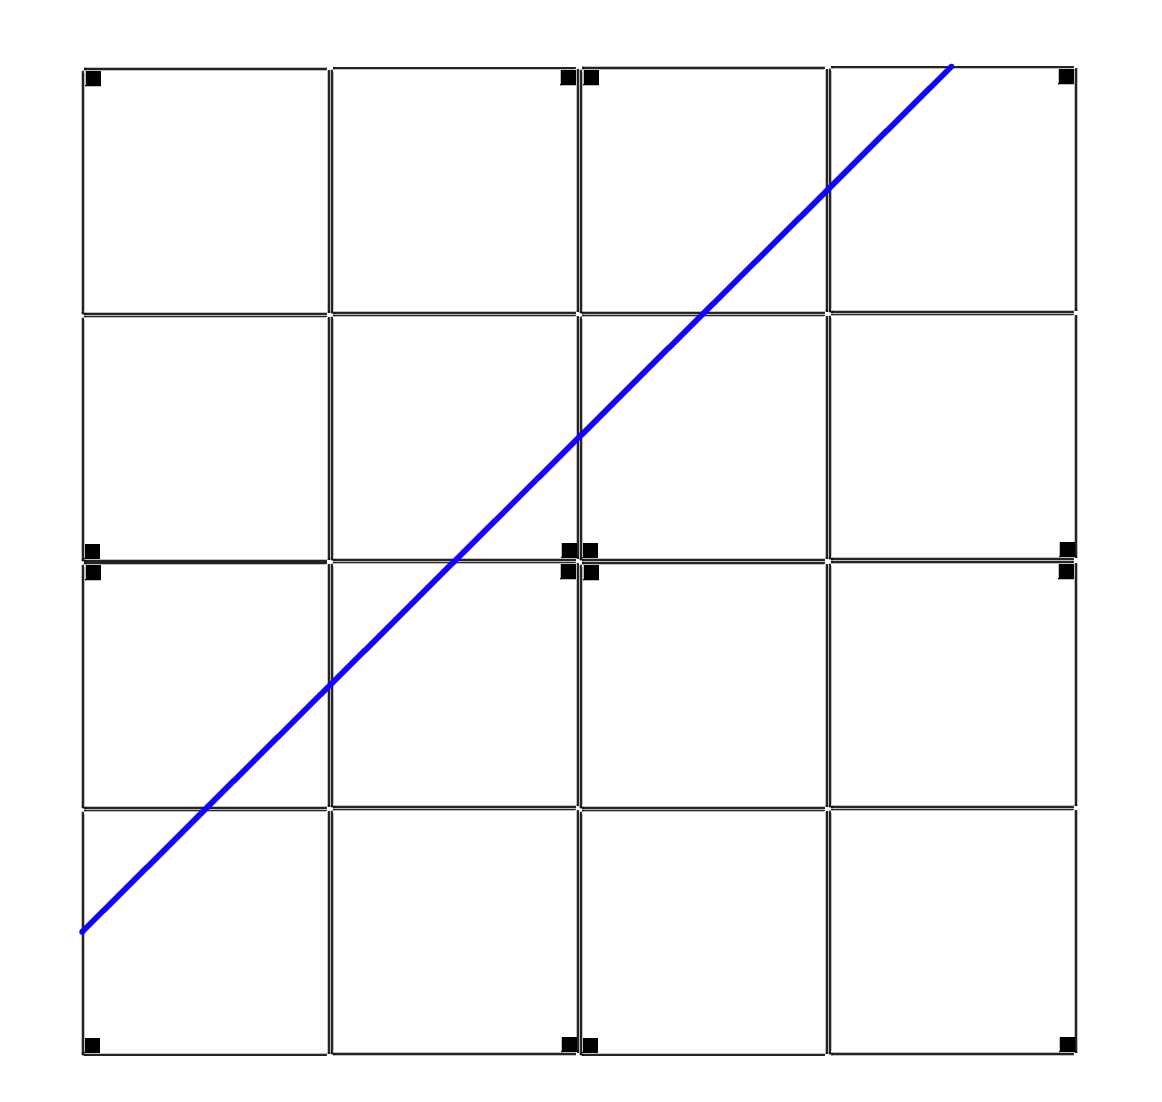
\includegraphics[width=1.7in]{tiling.png}
      \end{figure}
    \end{column}
  \end{columns}
}

\frame{
  \frametitle{Representing Collision Strings}

  \begin{example}
    Tiling of $\vec{x}_0 = (0, 0.5)$ and $\vec{v} = (0.25, 0.25)$.
  \end{example}

  \begin{columns}
    \begin{column}{0.45\textwidth}
      \begin{figure}
        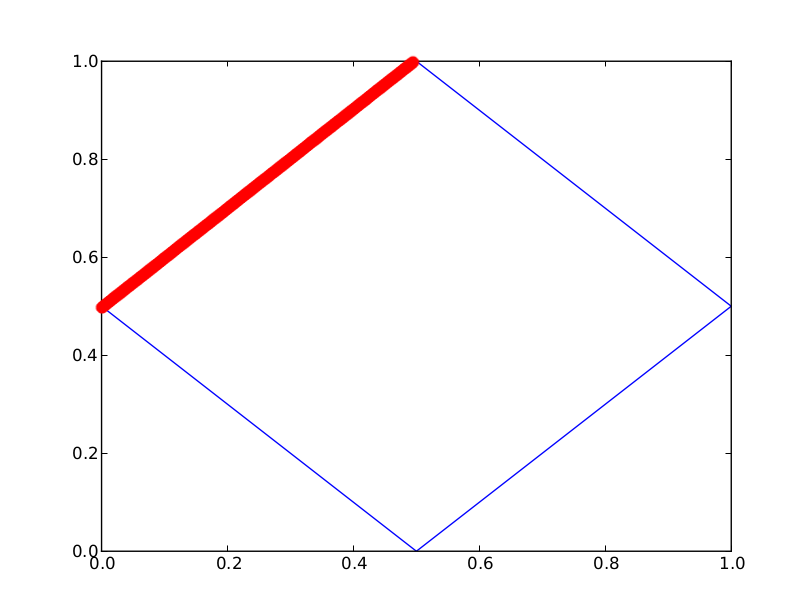
\includegraphics[width=2.1in]{tiling_real_step_1.png}
      \end{figure}
    \end{column}
    \begin{column}{0.45\textwidth}
      \begin{figure}
        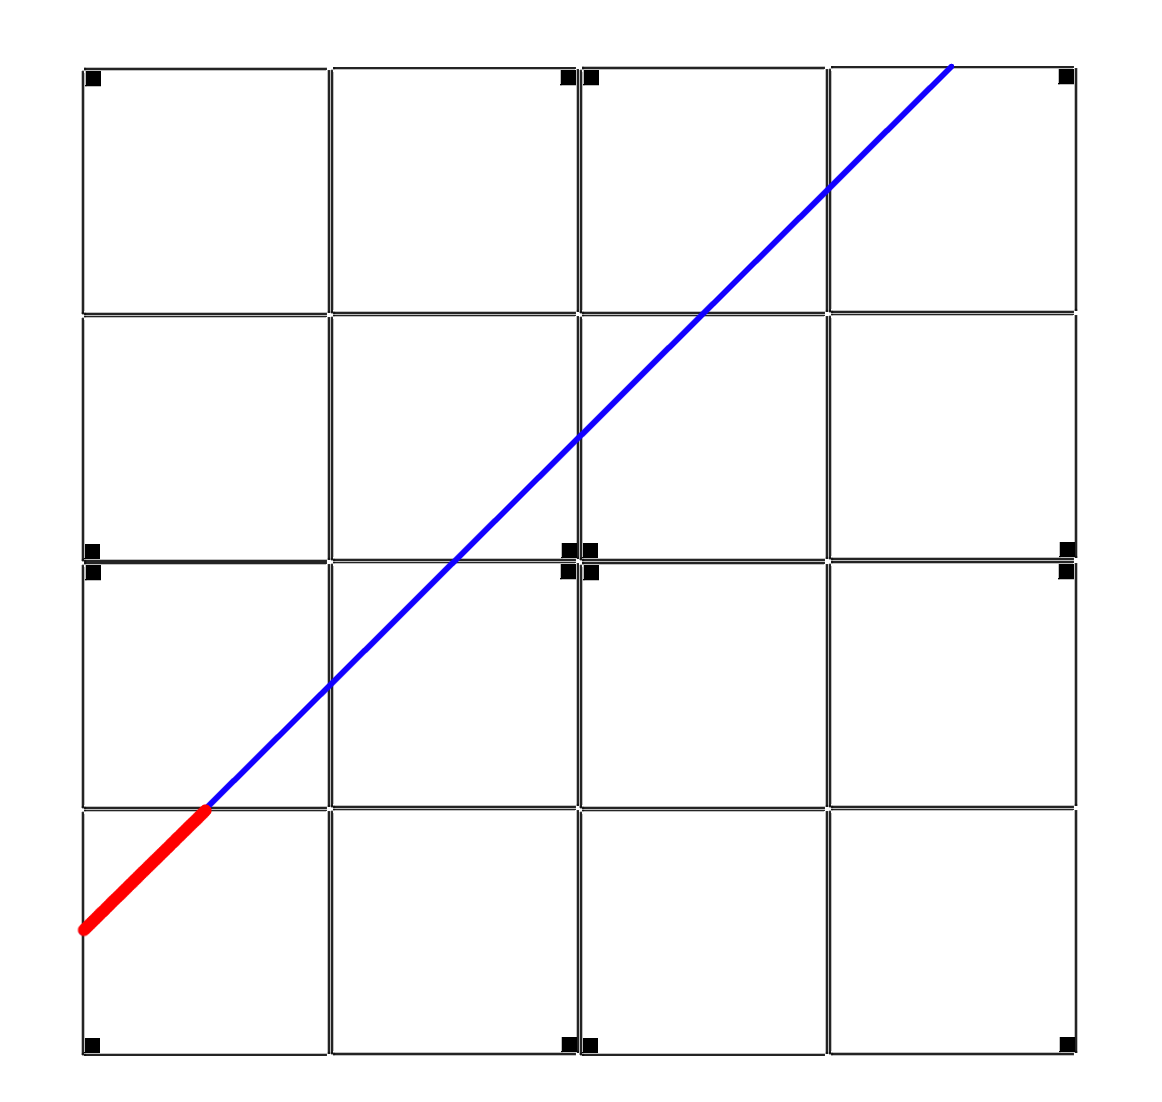
\includegraphics[width=1.7in]{tiling_tiled_step_1.png}
      \end{figure}
    \end{column}
  \end{columns}
}

\frame{
  \frametitle{Representing Collision Strings}

  \begin{example}
    Tiling of $\vec{x}_0 = (0, 0.5)$ and $\vec{v} = (0.25, 0.25)$.
  \end{example}

  \begin{columns}
    \begin{column}{0.45\textwidth}
      \begin{figure}
        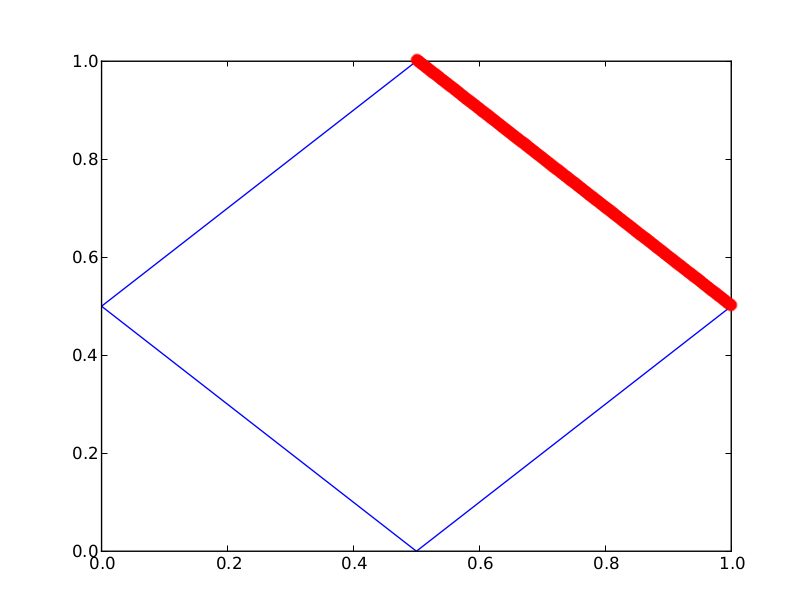
\includegraphics[width=2.1in]{tiling_real_step_2.png}
      \end{figure}
    \end{column}
    \begin{column}{0.45\textwidth}
      \begin{figure}
        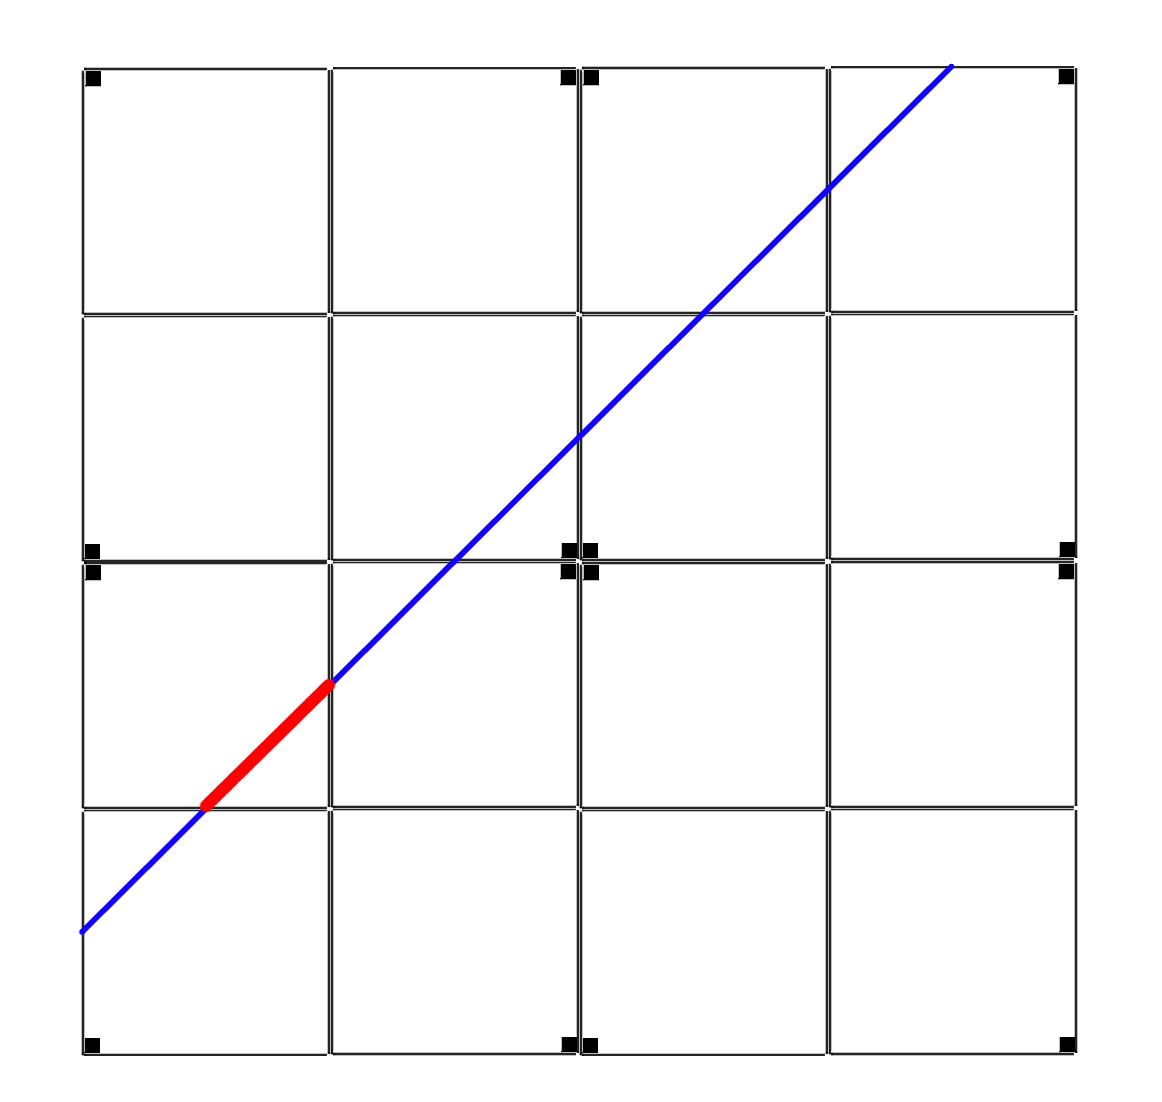
\includegraphics[width=1.7in]{tiling_tiled_step_2.png}
      \end{figure}
    \end{column}
  \end{columns}
}

\frame{
  \frametitle{Representing Collision Strings}

  \begin{example}
    Tiling of $\vec{x}_0 = (0, 0.5)$ and $\vec{v} = (0.25, 0.25)$.
  \end{example}

  \begin{columns}
    \begin{column}{0.45\textwidth}
      \begin{figure}
        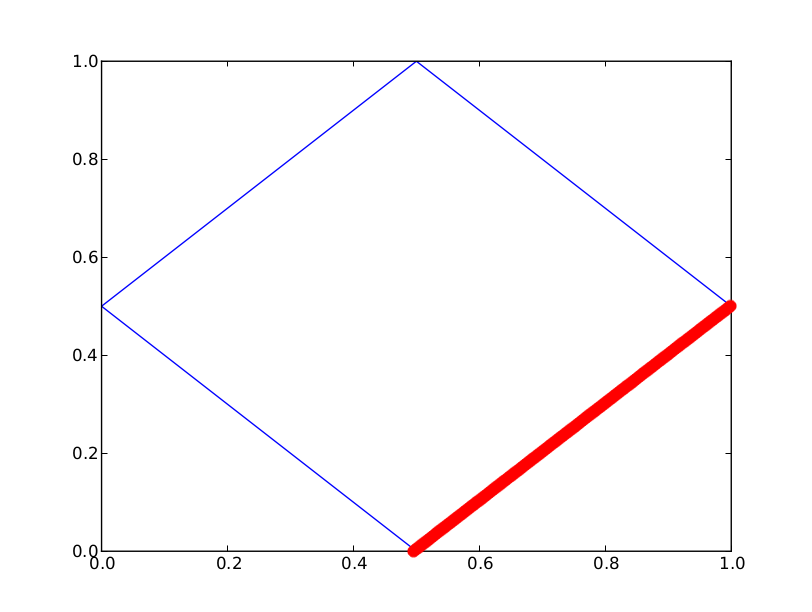
\includegraphics[width=2.1in]{tiling_real_step_3.png}
      \end{figure}
    \end{column}
    \begin{column}{0.45\textwidth}
      \begin{figure}
        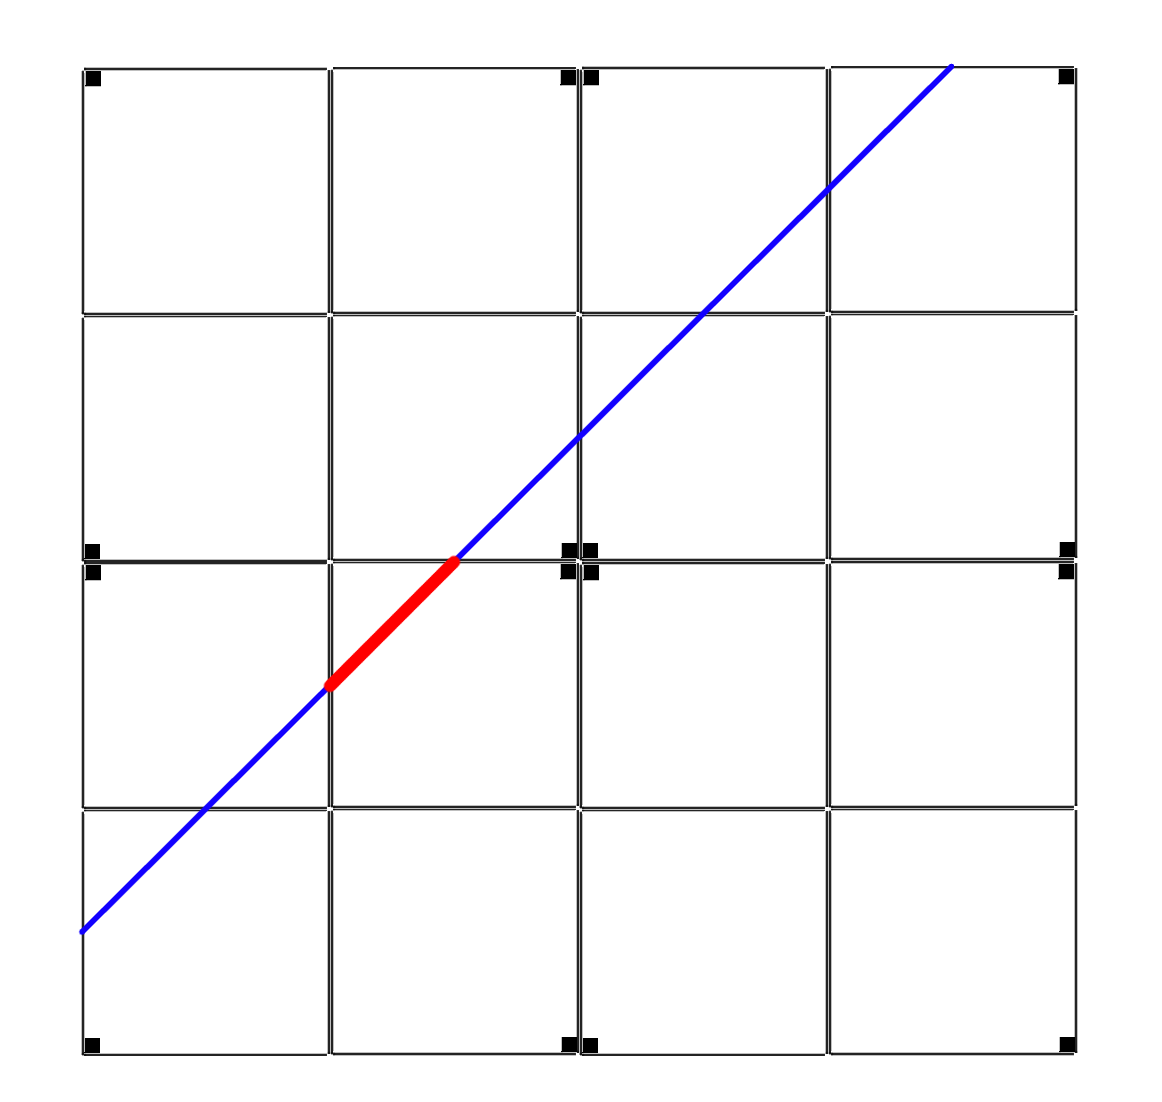
\includegraphics[width=1.7in]{tiling_tiled_step_3.png}
      \end{figure}
    \end{column}
  \end{columns}
}

\frame{
  \frametitle{Representing Collision Strings}

  \begin{example}
    Tiling of $\vec{x}_0 = (0, 0.5)$ and $\vec{v} = (0.25, 0.25)$.
  \end{example}

  \begin{columns}
    \begin{column}{0.45\textwidth}
      \begin{figure}
        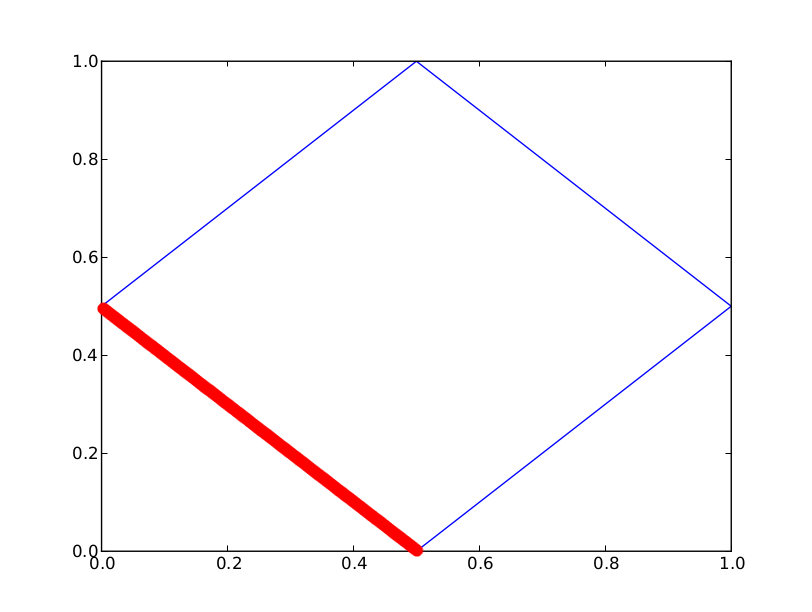
\includegraphics[width=2.1in]{tiling_real_step_4.png}
      \end{figure}
    \end{column}
    \begin{column}{0.45\textwidth}
      \begin{figure}
        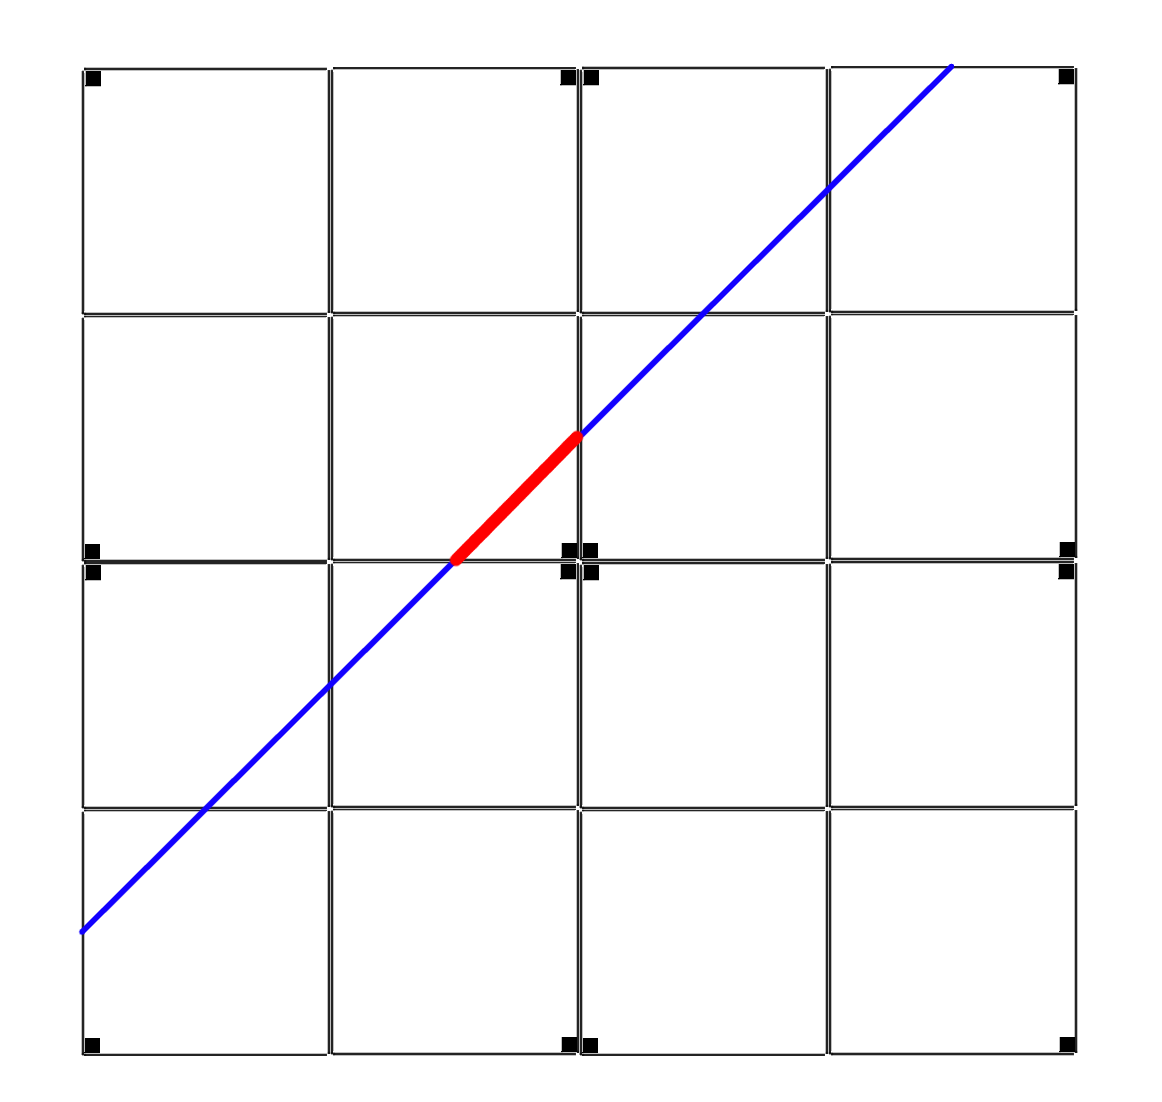
\includegraphics[width=1.7in]{tiling_tiled_step_4.png}
      \end{figure}
    \end{column}
  \end{columns}
}

\frame{
  \frametitle{Representing Collision Strings}

  \begin{example}
    Tiling of $\vec{x}_0 = (0, 0.5)$ and $\vec{v} = (0.25, 0.25)$.
  \end{example}

  \begin{columns}
    \begin{column}{0.45\textwidth}
      \begin{figure}
        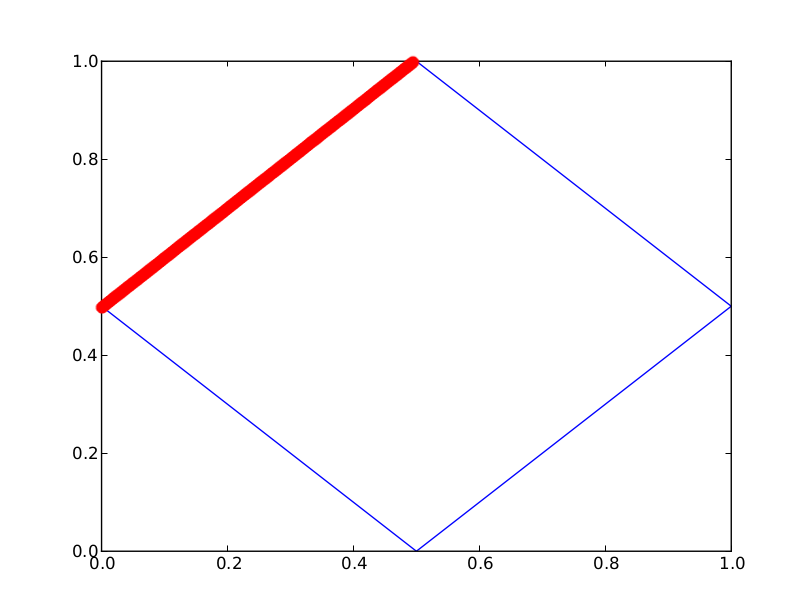
\includegraphics[width=2.1in]{tiling_real_step_1.png}
      \end{figure}
    \end{column}
    \begin{column}{0.45\textwidth}
      \begin{figure}
        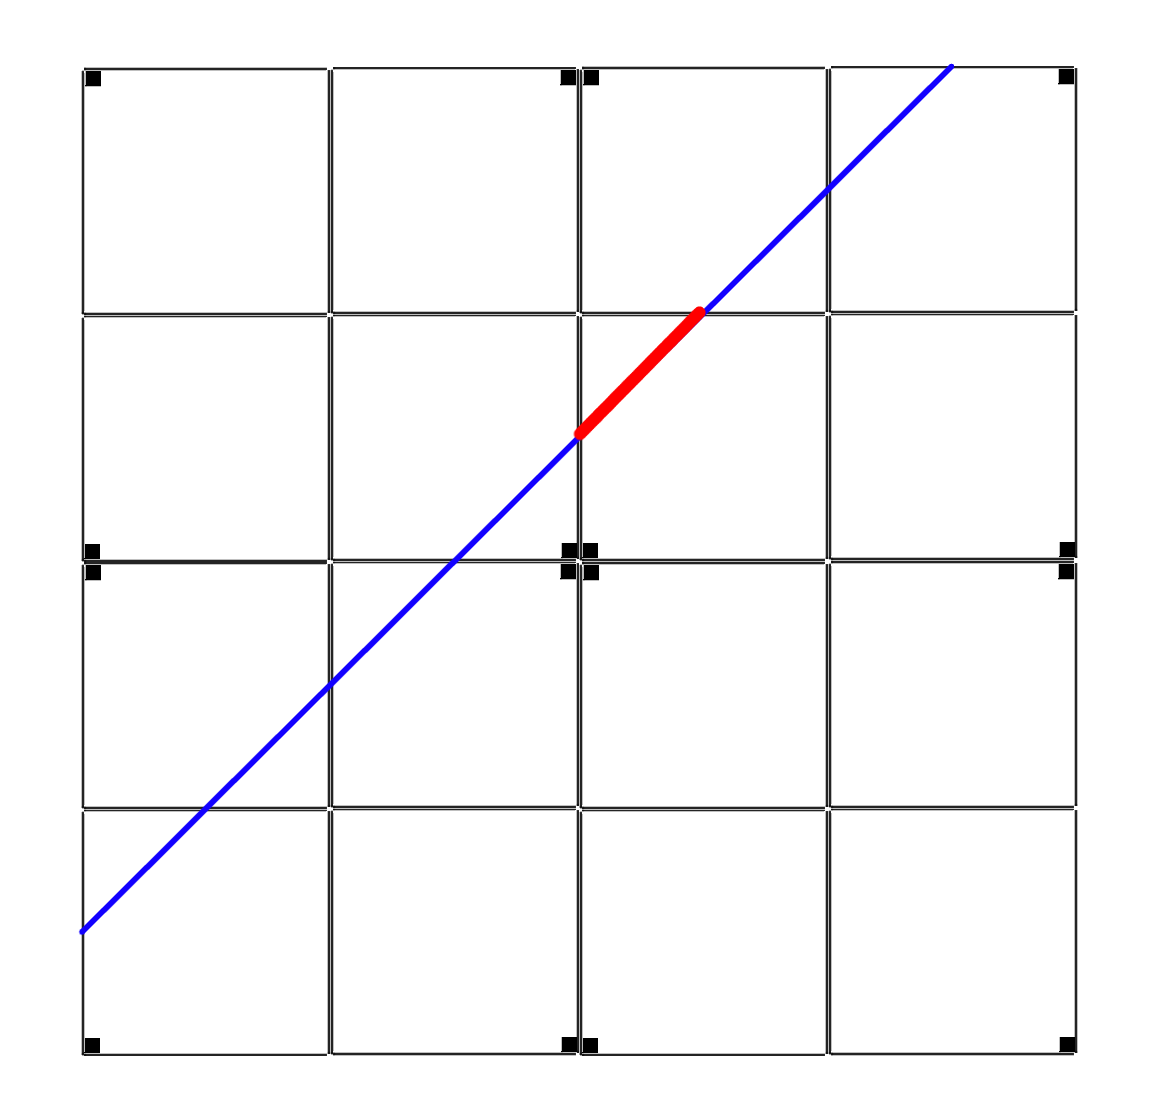
\includegraphics[width=1.7in]{tiling_tiled_step_5.png}
      \end{figure}
    \end{column}
  \end{columns}
}

\frame{
  \frametitle{Representing Collision Strings}

  \begin{example}
    Tiling of $\vec{x}_0 = (0, 0.5)$ and $\vec{v} = (0.25, 0.25)$.
  \end{example}

  \begin{columns}
    \begin{column}{0.45\textwidth}
      \begin{figure}
        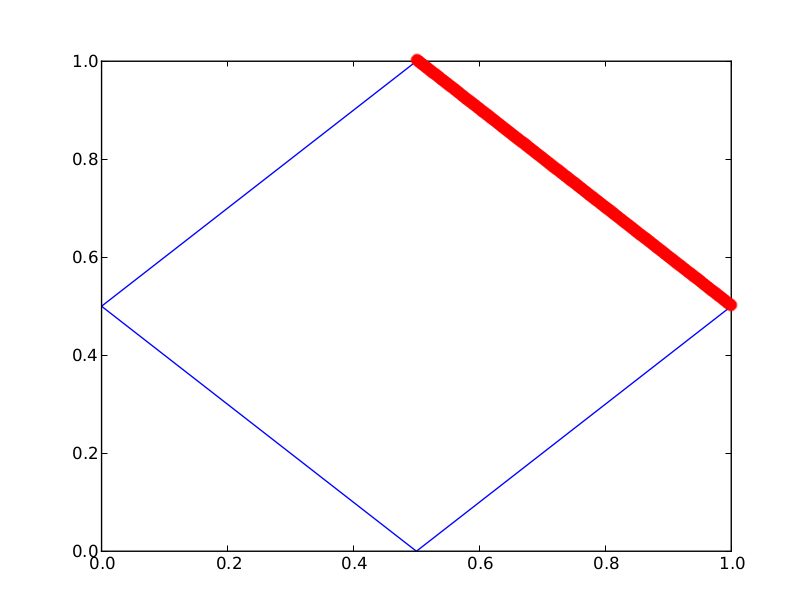
\includegraphics[width=2.1in]{tiling_real_step_2.png}
      \end{figure}
    \end{column}
    \begin{column}{0.45\textwidth}
      \begin{figure}
        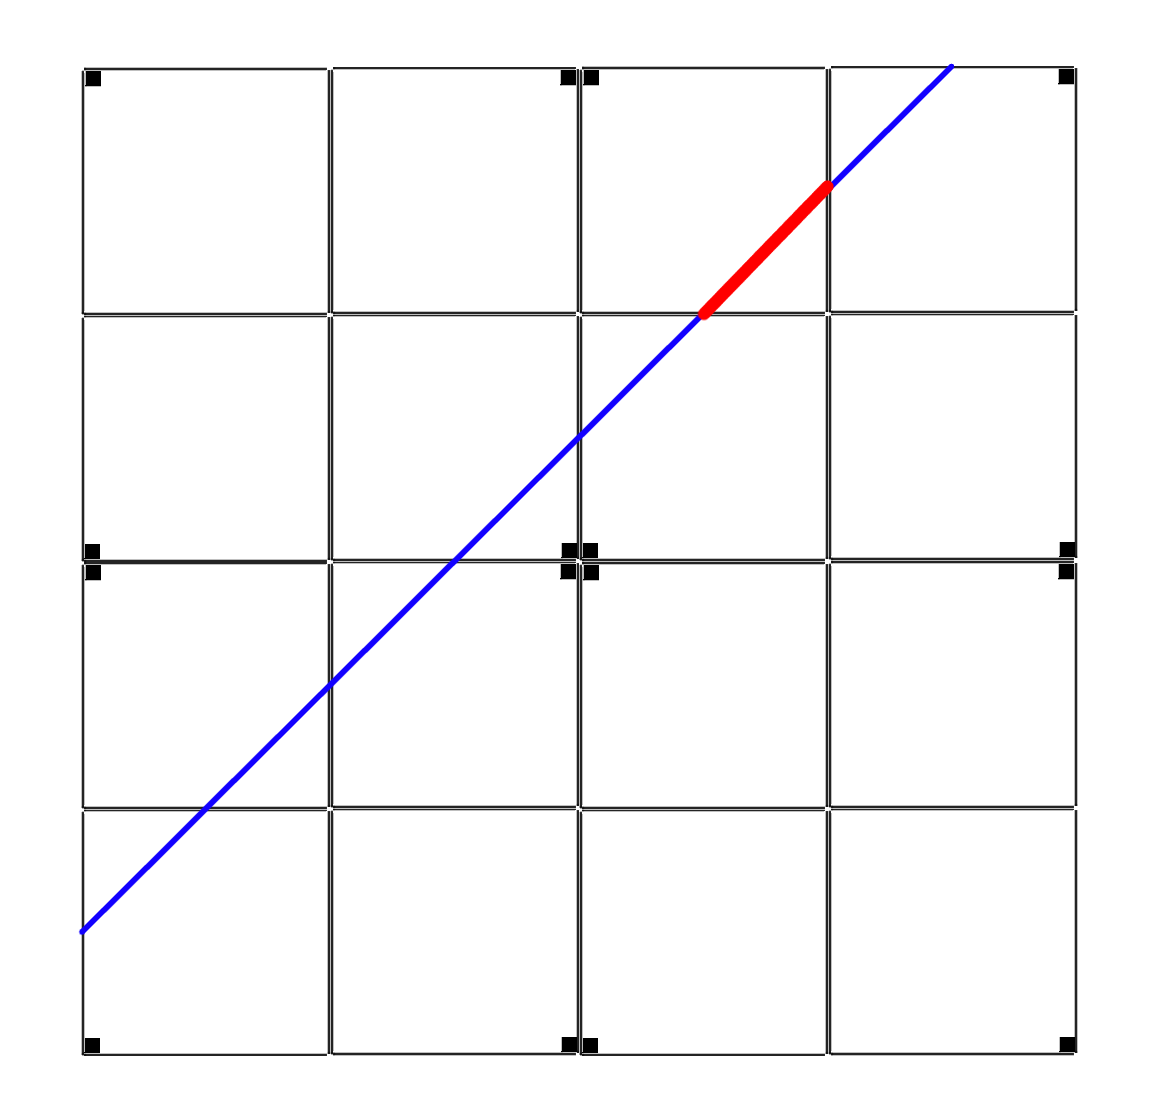
\includegraphics[width=1.7in]{tiling_tiled_step_6.png}
      \end{figure}
    \end{column}
  \end{columns}
}

\frame{
  \frametitle{Representing Collision Strings}

  \begin{example}
    Tiling of $\vec{x}_0 = (0, 0.5)$ and $\vec{v} = (0.25, 0.25)$.
  \end{example}

  \begin{columns}
    \begin{column}{0.45\textwidth}
      \begin{figure}
        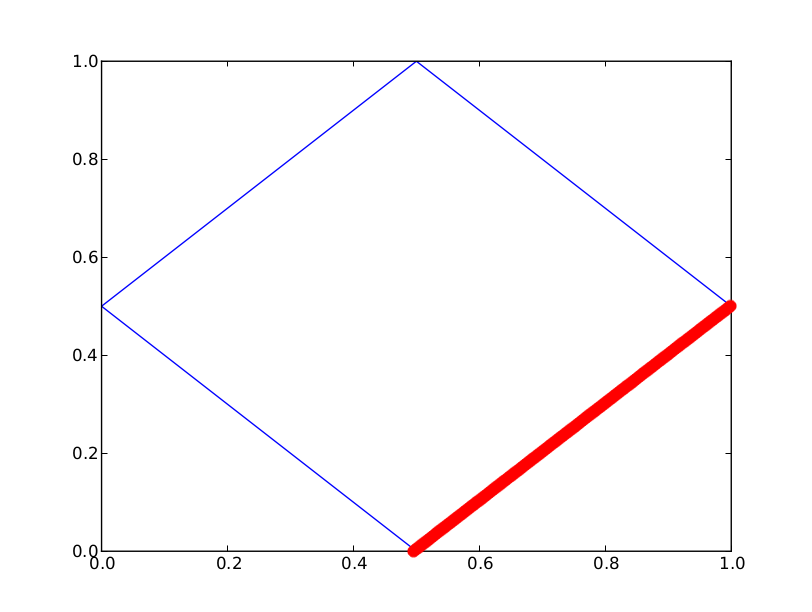
\includegraphics[width=2.1in]{tiling_real_step_3.png}
      \end{figure}
    \end{column}
    \begin{column}{0.45\textwidth}
      \begin{figure}
        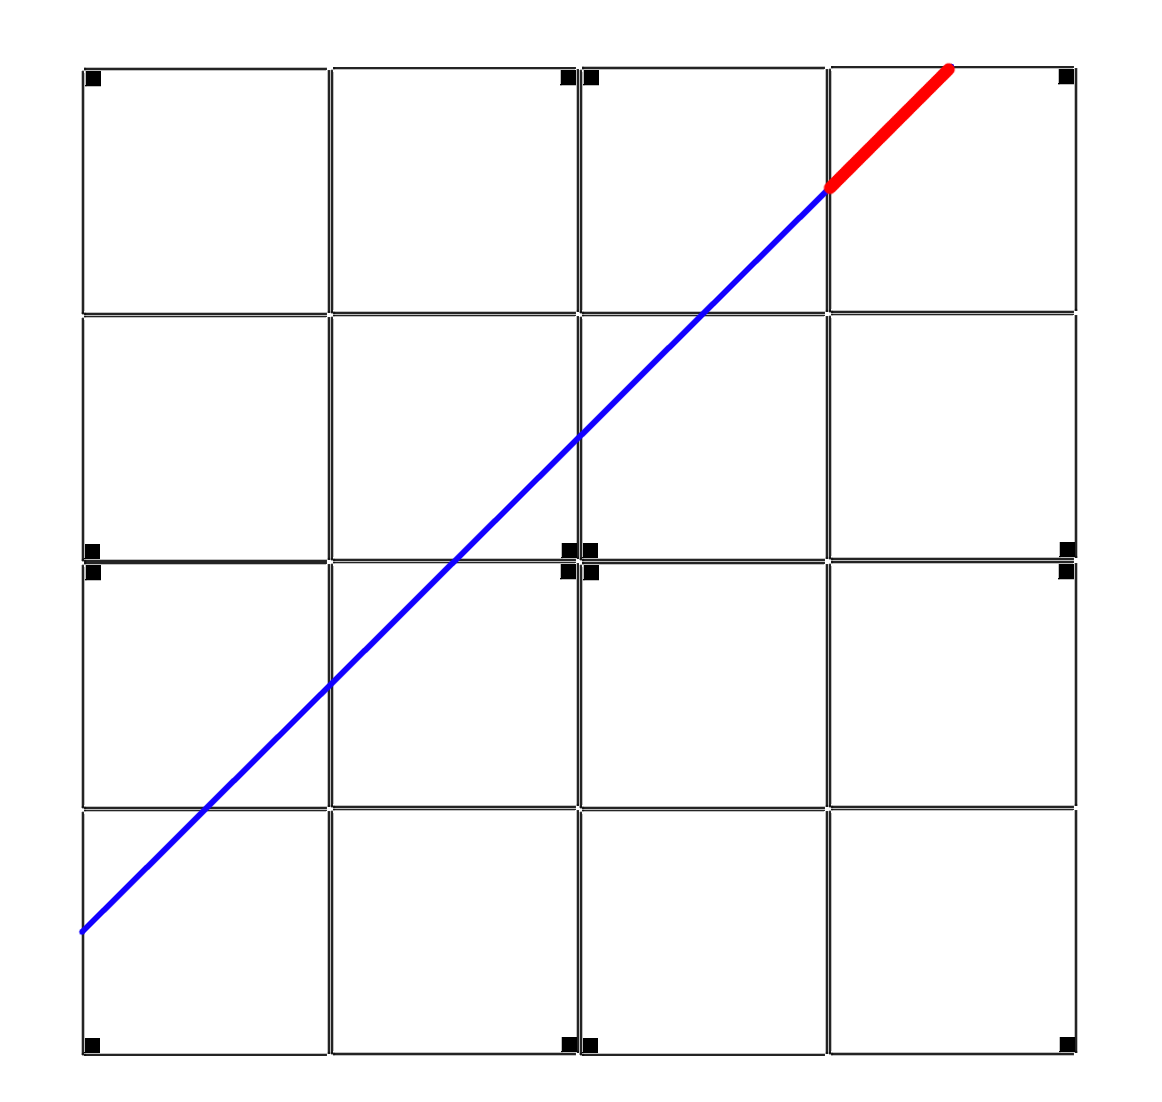
\includegraphics[width=1.7in]{tiling_tiled_step_7.png}
      \end{figure}
    \end{column}
  \end{columns}
}

\frame{
  \frametitle{Periodicity of Rationals}

  We can represent a particle as a line in the plane $y = mx + y_0$ in the tiling.

  Periodicity occurs if $y_0 2k = mx + y_0$ for some $k \in \mathrm{N}$.

  \begin{itemize}
    \item If $m, y_0 \in \mathrm{Q}$, then all sequences are periodic.
    \item If $m$ or $y_0$ are irrational, then the sequences are not periodic.
  \end{itemize}
}

\frame{
  \frametitle{Maximum Differences between Primary Substring Lengths}

  Given a collision string, how different can primary substrings be?

  \begin{example}
    Is $abaaab$ possible?
  \end{example}
}

\frame{
  \frametitle{Maximum Differences between Primary Substring Lengths}

  Length of primary substring $i$ is given by:
  \begin{eqnarray*}
    L(i, m, y_0) = \floor*{\frac{i - y_0}{m}} - \floor*{\frac{i-1 - y_0}{m}}
  \end{eqnarray*}
}

\frame{
  \frametitle{Maximum Differences between Primary Substring Lengths}

  For $i, j \in \mathrm{N}$, $m \in [0,1]$, $y_0 \in [0,1]$, we will show:

  \begin{eqnarray*}
    \max_{i > j} L(i, m, y_0) - L(j, m, y_0) \leq 2
  \end{eqnarray*}
}

\frame{
  \frametitle{Maximum Differences between Primary Substring Lengths}

  \begin{lemma}
    \begin{eqnarray*}
      \floor*{a - x} + \floor*{b - x} = \floor*{a} - \floor*{b} + (\floor*{\fracp*{a} - \fracp*{x}} - \floor*{\fracp*{b} - \fracp*{x}})
    \end{eqnarray*}
  \end{lemma}

  \begin{eqnarray*}
  L(i, m, y_0) - L(j, m, y_0) &=& \left( \floor*{\frac{i}{m}} - \floor*{\frac{i-1}{m}} \right) + \left( \floor*{\frac{j}{m}} - \floor*{\frac{j-1}{m}} \right) \\
                              &+& \left( \floor*{\fracp*{\frac{i}{m}} - \fracp*{\frac{y_0}{m}}} - \floor*{\fracp*{\frac{i-1}{m}} - \fracp*{\frac{y_0}{m}}} \right) \\
                              &-& \left( \floor*{\fracp*{\frac{j}{m}} - \fracp*{\frac{y_0}{m}}} - \floor*{\fracp*{\frac{j-1}{m}} - \fracp*{\frac{y_0}{m}}} \right) 
  \end{eqnarray*}
}

\frame{
  \frametitle{Maximum Differences between Primary Substring Lengths}

  Let $g(x, m, y_0) = \floor*{\fracp*{\frac{x}{m}} - \fracp*{\frac{y_0}{m}}} - \floor*{\fracp*{\frac{x-1}{m}} - \fracp*{\frac{y_0}{m}}}$.

  \begin{eqnarray*}
  L(i,m,y_0) - L(j,m,y_0) &=& \fracp*{\frac{i-1}{m}} - \fracp*{\frac{i}{m}} - \left(\fracp*{\frac{j-1}{m}} - \fracp*{\frac{j}{m}} \right) \\
                          &+& g(i,m,y_0) - g(j,m,y_0)
  \end{eqnarray*}
}

\frame{
  \frametitle{Maximum Differences between Primary Substring Lengths}
  \begin{itemize}
    \item If $g(x,m,y_0) = 1$, then:
      \begin{eqnarray*}
        \fracp*{\frac{x-1}{m}} < \fracp*{\frac{y_0}{m}} < \fracp*{\frac{x}{m}}
      \end{eqnarray*}

      Which implies $0 < L(x,m,y_0) < 1$.

    \item If $g(x,m,y_0) = -1$, then:
      \begin{eqnarray*}
        \fracp*{\frac{x}{m}} < \fracp*{\frac{y_0}{m}} < \fracp*{\frac{x-1}{m}}
      \end{eqnarray*}

      Which implies $-1 < L(x,m,y_0) < 0$.

    \item If $g(x,m,y_0) = 0$, then:
      $-1 < L(x,m, y_0) < 1$.
  \end{itemize}
}

\frame{
  \frametitle{Maximum Differences between Primary Substring Lengths}

  \begin{eqnarray*}
    \max_{i > j} L(i,m,y_0) - L(j,m,y_0) \leq 2
  \end{eqnarray*}
}

\subsection{1-dimensional Problem}

\frame{
  \frametitle{Sequence Characterization}

  \begin{multline*}
    \begin{array}{cccccccccc}
      \underbrace{aaa} & b & \underbrace{aa} & b & \underbrace{aa} & b & \underbrace{aaa} & b & \underbrace{aa} & b \\
      3 && 2 && 2 && 3 && 2 &
    \end{array}\\
    \begin{array}{cccccccc}
      \underbrace{aa} & b & \underbrace{aaa} & b & \underbrace{aa} & b & \underbrace{aaa} & \dots \\
      2 && 3 && 2 && 3 & \dots
    \end{array}
  \end{multline*}
}

\frame{
  \frametitle{Sequence Characterization}

  \begin{gather*}
    \begin{array}{cccccccc}
      3 & \underbrace{22} & 3 & \underbrace{22} & 3 & \underbrace{2} & 3 & \dots\\ 
      & 2 && 2 && 1 & \dots
    \end{array}
  \end{gather*}
}
